\documentclass[11pt,oneside,american,czech]{article}
\usepackage[T1]{fontenc}
\usepackage[utf8]{inputenc}
\usepackage[a4paper]{geometry}
\geometry{verbose,tmargin=4cm,bmargin=2.5cm,lmargin=2cm,rmargin=2cm,headheight=0.8cm,headsep=1cm,footskip=1cm}
% footskip dává mezeru mezi číslování stránek a textem
\pagestyle{headings}
\setcounter{secnumdepth}{3}
\usepackage{url}
\usepackage{amsmath}
\usepackage{amsthm}
%\usepackage{amssymb}
\usepackage{graphicx}
\usepackage{setspace}
\usepackage{subfiles}
\usepackage{cite}
\usepackage{tikz}


% Packages for code snipets
\usepackage{verbatim}
\usepackage{listings}

% Settings for code coloring
\usepackage{xcolor}
\definecolor{codegreen}{rgb}{0,0.6,0}
\definecolor{codegray}{rgb}{0.5,0.5,0.5}
\definecolor{codepurple}{rgb}{0.58,0,0.82}
\definecolor{backcolour}{rgb}{0.95,0.95,0.92}

\lstdefinestyle{mystyle}{
	backgroundcolor=\color{backcolour},   
	commentstyle=\color{codegreen},
	keywordstyle=\color{codegreen},
	numberstyle=\tiny\color{codegray},
	stringstyle=\color{codepurple},
	basicstyle=\ttfamily\footnotesize,
	breakatwhitespace=false,         
	breaklines=true,                 
	captionpos=b,                    
	keepspaces=true,                 
	numbers=left,                    
	numbersep=5pt,                  
	showspaces=false,                
	showstringspaces=false,
	showtabs=false,                  
	tabsize=2
}
\lstset{style=mystyle}

\lstset{ % ... whatever was already there ...
	literate=% ... any other literates already there ...
	{!}{!}1
	{?}{?}1
	{:}{:}1
	{;}{;}1
}


% packages for tables, subtables and subfigures
\usepackage{booktabs}
\usepackage{multirow}
%\usepackage{subfig}

\usepackage{caption}
\usepackage{subcaption}

% hyperlinks
\usepackage[hidelinks]{hyperref}
\hypersetup{
	colorlinks=true,
	linkcolor=blue,
	filecolor=magenta,      
	urlcolor=cyan,
}

% Font
\usepackage[charter]{mathdesign}
\usepackage[format=hang]{caption}
%% Indent even the first paragraph in each section
\usepackage{indentfirst}

% completely avoid orphans (first lines of a new paragraph on the bottom of a page)
\clubpenalty=9500
% completely avoid widows (last lines of paragraph on a new page)
\widowpenalty=9500

\usepackage{babel}
\title{MMC - Gibbs sampler \& Hamiltonian Monte Carlo}
\author{Michaela Mašková}
\date{\today}

\newcommand{\E}{\mathbb{E}}
\newcommand{\N}{\mathcal{N}}
\newcommand{\der}{\mathrm{d}}
\newcommand{\G}{\mathcal{G}}
\newcommand{\half}{\frac{1}{2}}
\newcommand{\id}{\mathrm{I}}

\begin{document}
% Initial settings
\def\listingsfont{\ttfamily}

% make title
\maketitle

Protokol se zabývá použitím Monte Carlo metod pro bayesovské odhadování parametrů.

\tableofcontents

\section{Markov Chain Monte Carlo}

Monte Carlo metody je možné použít na nejrůznější typy úloh -- výpočet integrálů, diferenciálních rovnic atd. V pravděpodobnostních úlohách často počítáme střední hodnoty, které jsou právě integrálem typu
\begin{equation*}
\E_{ x \sim U(0,1)} \left[ f(x) \right] = \int_0^1 f(x) U(0,1) \der x.
\end{equation*}
Střední hodnotu, tedy daný integrál, je pak možné odhadnout metodou Monte Carlo, nicméně musíme být schopní generovat náhodně z příslušné hustoty pravděpodobnosti. Pokud tedy máme například pouze naměřená data, která pochází z nějakého modelu, musíme nejdřív získat jejich distribuci a teprve poté z ní můžeme generovat náhodné vzorky, abychom spočítali příslušnou střední hodnotu. Problém nastává, pokud příslušná rozdělení není možné spočítat analyticky -- což bude přesně případ našich modelových příkladů.

V tomto protokolu budeme používat dvě Monte Carlo metody
\begin{itemize}
	\item Gibbs sampler
	\item Hamiltonian Monte Carlo.
\end{itemize}
Obě vychází z Markov Chain Monte Carlo.

\subsection{Metropolis Hastings a Gibbs sampler}
Metropolisův algoritmus funguje na následujícím principu: Místo konkrétní distribuce zvolíme Markovův řetězec, který bude konvergovat k hledané distribuci. Postup má pak následující kroky
\begin{enumerate}
	\item Vybereme kernel $q(\theta | \theta^{(i)})$.
	\item Vygenerujeme vzorek $\theta^* \sim q(\theta | \theta^{(i)})$.
	\item S pravděpodobností
	\begin{equation*}
	\min \left[ 1, \frac{p(\theta^{*})q(\theta^{(i)}|\theta^{*})}{p(\theta^{(i)}) q(\theta^*|\theta^{(i)})} \right]
	\end{equation*}
	přijímáme $\theta^{*}$: $i \leftarrow i + 1, \theta^{(i)} \leftarrow \theta^{*}$, jinak zamítáme a vracíme se do bodu 2.
\end{enumerate}

Zvoleným kernelem je nějaká náhodná procházka (Gaussův proces) s parametry $\phi$.

\textbf{Gibbs sampler} je speciální vícedimenzionální podoba MCMC -- Metropolis Hastings algoritmu. Pro distribuce tvaru
\begin{equation*}
p(\theta_1, \theta_2, \dots, \theta_k)
\end{equation*}
jsou vzorky generovány postupně jako
\begin{align*}
\text{1.} & \quad \theta_1^{(i+1)} \sim p(\theta_1|\theta_2^{(i)}, \dots, \theta_k^{(i)}) \\
\text{2.} & \quad \theta_2^{(i+1)} \sim p(\theta_2|\theta_2^{(i+1)}, \dots, \theta_k^{(i)}) \\
& \vdots \\
\text{k.} & \quad \theta_k^{(i+1)} \sim p(\theta_k|\theta_1^{(i+1)}, \dots, \theta_{k-1}^{(i+1)}),
\end{align*}
kde pravděpodobnost přijetí je 1.


\subsection{Hamiltonian Monte Carlo}

Hamiltonovské Monte Carlo se jmenuje podle hamiltoniánu. Tato metoda totiž pracuje tak, že si vezme logaritmus hustoty pravděpodobnosti jako potenciální energii
\begin{equation*}
	U(\theta) = - \log p(\theta) = \frac{\theta^2}{2}.
\end{equation*}
Dále zavedeme kinetickou energii v proměnné $p$ (hybnost)
\begin{equation*}
	K(p) = \frac{p^2}{2}.
\end{equation*}
Hamiltonovy rovnice říkají, že
\begin{equation*}
	\frac{\der x_i}{\der t} = \frac{\partial H}{\partial p_i} \quad \text{a} \quad \frac{\der p_i}{\der t} = - \frac{\partial H}{\partial x_i},
\end{equation*}
kde $x_i, p_i$ jsou i-té komponenty polohy a hybnosti. Jako polohu tedy bereme hledaný parametr $\theta$. Samotný hamiltonián pak má tvar $H(\theta, p) = U(\theta) + \half mp^2$ a dostáváme
\begin{equation*}
	\frac{\der \theta}{\der t} = p \quad \text{a} \quad \frac{\der p}{\der t} = -\theta.
\end{equation*}

Úloha se tak převede na simulaci diferenciálních rovnic pro vybrané časy $t = 0, \dots, t_N$. Vyžadujeme tak nějaké číslo $L$, což je počet skoků pro \textit{leapfrog} algoritmus. Na začátku vygenerujeme náhodně hybnost $p^0 \sim \N(0,m)$ a řešíme hamiltonovské rovnice. Pro řešení těchto rovnic se používá numerická metoda \textit{leapfrog integration}. Vždy po $\Delta t$ časovém úseku jsou pak spočítány nové hodnoty $\theta$ a $p$.

HMC asymtoticky konverguje k pravé distribuci a navíc výsledné $\theta^{*}$ je nezávislé na $p^{*}$. Tuto metodu nebudeme implementovat přímo, ale využijeme balíček Turing.jl pro pravděpodobnostní programování, kde už je algoritmus naimplementován.

\subsection{Porovnání metod}
Metoda Gibbs sampleru je už ze zápisu jednodušší na implementaci a navíc vychází z klasické bayesovské inference, což nám umožňuje ji jednoduše využít na řadu různých problémů. Nicméně jednotlivé náhodně vybírané hodnoty jsou určitým způsobem korelované -- závisí vždy na předchozím výsledku. HMC tuto nevýhodu eliminuje, čímž dokáže rychleji prozkoumat zkoumaný prostor proměnných. Nevýhodou HMC je však naopak výpočetní náročnost --  použitím této metody v podstatě zdvojnásobujeme počet proměnných (přidáváme do modelu hybnost).

\newpage
\section{Definice problému a odvození algoritmu}

Ve statistice se často snažíme najít odhady parametrů. V bayesovském přístupu však hledaný parametr neodhadujeme bodově jako v klasické statistice. Nehledáme tedy například odhad dané veličiny jako průměr nebo jinou statistiku, ale snažíme se najít pravděpodobnostní rozdělení daných parametrů.

\subsection{Toy problem}
Představme si, že máme 2 hodnoty $x_i$, které jsou generovány z rozdělení $p(x | m, s) = \N(x | m, s)$, kde $m$ a $s$ jsou neznámé parametry. Bayesovský přístup spočívá v zavedení tzv. apriorního rozdělení přes tyto hledané parametry. Zde zvolíme jako apriorní rozdělení následující:
\begin{itemize}
	\item $p(m) = \N(m | \mu, \phi)$
	\item $p(s) = i \G(s | \alpha, \beta)$.
\end{itemize}
Počítáme s tím, že $\alpha, \beta, \phi$ a $\mu$ jsou hyperparametry -- tedy jejich hodnoty fixujeme na předem zvolených číslech. Grafickou strukturu takového modelu si můžeme prohlédnout na Obr. \ref{Obr: Model}.


\begin{figure}[h!]
	\centering
	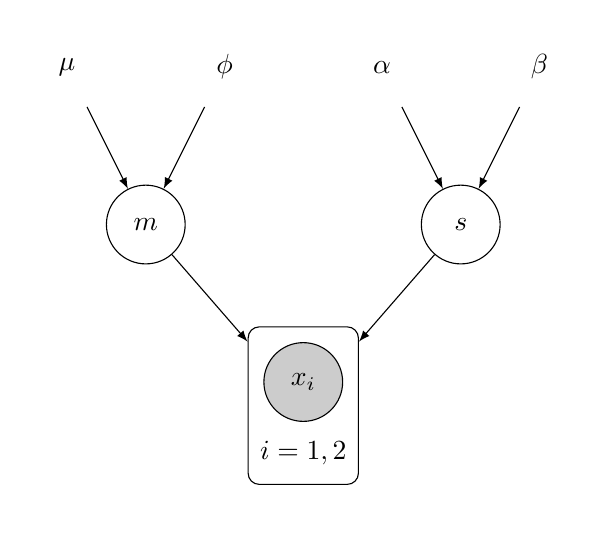
\begin{tikzpicture}[node distance = 2cm, minimum height=1cm, minimum width=1cm]
	\node[](mu) {$\mu$};
	\node[right of=mu](phi) {$\phi$};
	\node[right of=phi](alpha) {$\alpha$};
	\node[right of=alpha](beta) {$\beta$};
	
	\node[draw, circle, below of=mu, xshift=1cm](m) {$m$};
	\node[draw, circle, below of=alpha, xshift=1cm](s) {$s$};
	\node[draw, circle, below of=m, xshift=2cm, fill=black!20](xi) {$x_i$};
	\node[draw, rectangle, rounded corners, below of=m, minimum height=2cm, minimum width=1.4cm, yshift=-0.3cm, xshift=2cm](xi kolem) {};
	\node[below of=m, minimum height=2cm, minimum width=1.2cm, yshift=-0.9cm, xshift=2cm](xi kolem text) {$i = 1,2$};
	
	\draw[-latex] (mu) -- (m);
	\draw[-latex] (phi) -- (m);
	\draw[-latex] (alpha) -- (s);
	\draw[-latex] (beta) -- (s);
	\draw[-latex] (m) -- (xi kolem);
	\draw[-latex] (s) -- (xi kolem);
	\end{tikzpicture}
	\caption{Bayesovský model pro toy problem $(*)$.}
	\label{Obr: Model}
\end{figure}

Problém však je v tom, že v takto definovaném modelu nedokážeme analyticky najít marginální rozdělení pro $m$ a $s$, kde by jeden parametr nebyl závislý na druhém. Ani s pevnou volbou parametrů $\alpha, \beta$ a $\mu, \phi$ tak nedokážeme analyticky naleznout hustoty rozdělení $p(m)$ a $p(s)$.

Proto použijeme metodu Monte Carlo.


\subsubsection*{Odvození pro Gibbs sampler}

Pro odvození tvarů příslušných podmíněných marginálních rozdělení využijeme toho, že porovnáme jednotlivé tvary podle bayesovy věty ve tvaru
\begin{equation*}
p(\theta|x, \alpha) \propto p(x| \theta)p(\theta|\alpha),
\end{equation*}
kde $\theta$ jsou hledané parametry a $\alpha$ představuje parametry apriorních rozdělení (hyperparametry).

Použitím pro tento konkrétní příklad dostáváme

\begin{equation}
	p(m,s| x_1,x_2,\mu, \alpha, \beta, \Phi) \propto \prod_{i=1}^{2} p(x_i,m,s)p(m|\mu,\Phi)p(s|\alpha,\beta)
\end{equation}

a úpravou pak získáme
\begin{align*}
p(m,s|x_1,x_2,\mu, \alpha, \beta, \phi) & \propto \frac{1}{s} \frac{1}{s^{\alpha+1}} \exp \left[ - \frac{1}{2} \frac{(m - x_1)^2}{s} - \frac{1}{2} \frac{(m - x_1)^2}{s} \frac{1}{2} \frac{(m - \mu)^2}{\phi} - \frac{\beta}{s} \right] \\
p(m|s,x_1,x_2,\mu, \alpha, \beta, \phi) & \propto \frac{1}{s} \frac{1}{s^{\alpha+1}} \exp \left[ - \frac{1}{2} \frac{(m - x_1)^2}{s} - \frac{1}{2} \frac{(m - x_1)^2}{s} \frac{1}{2} \frac{(m - \mu)^2}{\phi} \right] \\
& \propto \exp \left[ - \frac{1}{2}\left( m^2 \left( \frac{1}{\phi} + \frac{2}{s} \right) \right) - 2m \left( \frac{\mu}{\phi} + \frac{x_1 + x_2}{s} \right) \right] \\
& = \N \left( m \; \big| \; \left( \frac{1}{\phi} + \frac{2}{s} \right)^{-1} \left( \frac{\mu}{\phi} + \frac{x_1 + x_2}{s} \right),  \left( \frac{1}{\phi} + \frac{2}{s} \right)^{-1} \right) \\
p(s|m,x_1,x_2,\mu, \alpha, \beta, \phi) & \propto  \exp \left[ - \frac{1}{2} \frac{(m - x_1)^2}{s} - \frac{1}{2} \frac{(m - x_1)^2}{s} - \frac{\beta}{s} \right] \\
& = i \G \left( s \big| \alpha + 1, \half(m - x_1)^2 + \half (m - x_2)^2 + \beta \right)
\end{align*}

Algoritmus pak bude iterativně probíhat pro $i = 1:K$, kde $K$ je celkový počet opakování podle vzorců
\begin{align}
	m^{(i+1)} & \sim \N \left( m \; \big| \; \left( \frac{1}{\phi} + \frac{2}{s^{(i)}} \right)^{-1} \left( \frac{\mu}{\phi} + \frac{x_1 + x_2}{s^{(i)}} \right),  \left( \frac{1}{\phi} + \frac{2}{s^{(i)}} \right)^{-1} \right) \label{Eq: Toy Gibbs m}\\
	s^{(i+1)} & \sim i \G \left( s \big| \alpha + 1, \half(m^{(i+1)} - x_1)^2 + \half (m^{(i+1)} - x_2)^2 + \beta \right)	\label{Eq: Toy Gibbs s}
\end{align}

\subsection{Bayesovská lineární regrese}
I lineární regresi je možné řešit bayesovsky. V takovém případě předpokládáme, že existuje lineární závislost ve tvaru
\begin{equation*}
	\boldsymbol{y} = \theta \cdot \boldsymbol{X} + \boldsymbol{e},
\end{equation*}
kde $\boldsymbol{X}$ je matice sestavená z vektorů $\boldsymbol{x}$ a $\theta$ je vektor příslušných regresních parametrů. Vektor $\boldsymbol{e}$ je pak gaussovský náhodný šum.

Pro lineární regresi sestavíme pravděpodobnostní model ve tvaru
\begin{equation*}
	p(\boldsymbol{y}, \theta | \boldsymbol{X}, \alpha) = p(\boldsymbol{y} | \theta, \boldsymbol{X}, \omega) p(\theta |\alpha) = \N (\boldsymbol{X} \theta, \omega \id) \N (0,\alpha^{-1} \id) \propto \exp \left[ - \half \omega ||\boldsymbol{y} - \boldsymbol{X} \theta ||^2 - \half \alpha || \theta ||^2 \right].
\end{equation*}
Této metodě se také říká Ridge Regression a řeší problém, kdy matice $X$ vede k nestabilitě numerické metody řešení.

Pokračujeme v bayesovském přístupu a zavedeme příslušné apriorní rozdělení pro $\alpha = G(\delta, \gamma)$. Parametr $\alpha$ zde zastává úlohu určitého regularizačního členu, který zabraňuje přefitování a vysokým hodnotám parametrů $\theta_i$. Schéma modelu je pak vidět na Obr. \ref{Obr: Model 2}.

\begin{figure}[h!]
	\centering
	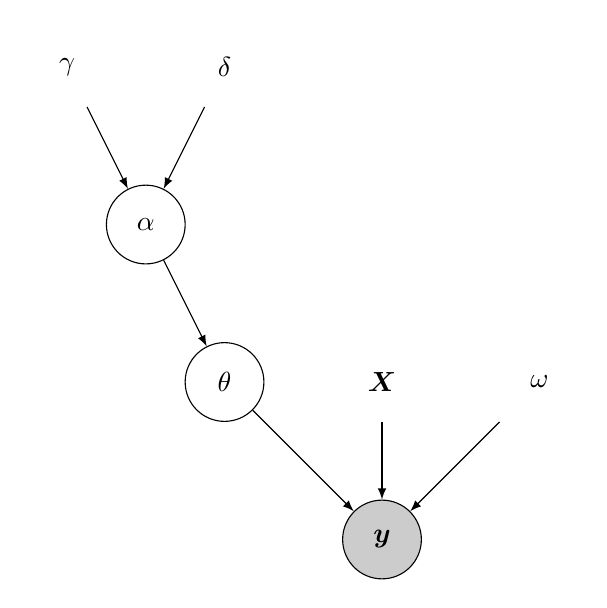
\begin{tikzpicture}[node distance=2cm, minimum height=1cm, minimum width=1cm]
		\node[] (gamma) {$\gamma$};
		\node[right of=gamma] (delta) {$\delta$};
		\node[draw, circle, below of=gamma, xshift=1cm] (alpha) {$\alpha$};
		\node[draw, circle, below of=alpha, xshift=1cm] (theta) {$ \theta$};
		\node[right of=theta] (X) {$\boldsymbol{X}$};
		\node[right of=X] (omega) {$\omega$};
		\node[draw, circle, fill=black!20, below of=X] (y) {$\boldsymbol{y}$};
		
		\draw[-latex] (gamma) -- (alpha);
		\draw[-latex] (delta) -- (alpha);
		\draw[-latex] (alpha) -- (theta);
		\draw[-latex] (theta) -- (y);
		\draw[-latex] (X) -- (y);
		\draw[-latex] (omega) -- (y);
	\end{tikzpicture}
	\caption{Bayesovský model pro lineární regresi $(+)$.}
	\label{Obr: Model 2}
\end{figure}

\subsubsection*{Odvození pro Gibbs sampler}

Stejně jako v toy problemu si spočítáme podmíněné distribuce pro $\theta$ a $\alpha$. Sdružená hustota pravděpodobnosti má tvar
\begin{align*}
	p(\boldsymbol{y}, \theta, \alpha |\boldsymbol{X}) & = p(\boldsymbol{y} | \theta, \boldsymbol{x}, \omega)p(\theta | \alpha)p(\alpha) = \N(\boldsymbol{X} \theta, \omega \id) \N(0,\alpha^{-1} \id) G(\delta, \gamma)  \\
	\implies p(\theta, \alpha |\boldsymbol{y}, \boldsymbol{X}) & \propto \alpha^{\delta + d/2 - 1} \exp \left[ - \half \omega ||\boldsymbol{y} - \boldsymbol{X} \theta ||^2 - \half \alpha || \theta ||^2 - \gamma \alpha  \right]
\end{align*}
a tedy jednotlivé marginální hustoty pravděpodobnosti závislé na příslušných parametrech budou
\begin{align*}
	p(\theta | \alpha, \boldsymbol{y}, \boldsymbol{X}) & = \N \left( \hat{\theta}, \left( \boldsymbol{X}^T \boldsymbol{X} + \alpha \id \right)^{-1} \right) \\
	p(\alpha | \theta, \boldsymbol{y}, \boldsymbol{X}) & = \G \left(\delta + \frac{d}{2}, \gamma + ||\theta||^2 \right).
\end{align*}

Vzorce pro algoritmus Gibbs sampleru tak budou mít tvar
\begin{align}
	\theta^{(i+1)} & \sim \N \left( \hat{\theta}, \left( \boldsymbol{X}^T \boldsymbol{X} + \alpha^{(i)} \id \right)^{-1} \right) \label{Eq: Gibbs linreg m} \\
	\alpha^{(i+1)} & \sim \G \left(\delta + \frac{d}{2}, \gamma + ||\theta^{(i+1)}||^2 \right) \label{Eq: Gibbs linreg s}
\end{align}

\section{Julia language}
\subsection{Generátory náhodných čísel}

Julia language je programovací jazyk určený převážně pro vědecké výpočty se zaměřením hlavně na rychlost a jednoduchost.

Pro generování náhodných čísel z rozdělení $U(0,1)$ je použit Mersenne Twister s použitím speciální knihovny Merseen Twister Library. %(http://www.math.sci.hiroshima-u.ac.jp/m-mat/MT/SFMT/#dSFMT).
V protokolu je nutné generovat náhodná čísla z několika různých rozdělení. Generování z $\N(0,1)$ probíhá pomocí Zigurratova algoritmu. Pro získání rozdělení s jinou střední hodnotou nebo rozptylem jsou použity známé transformace rozdělení.

Julia má implementovány metody pro generování náhodných čísel z většiny běžně používaných rozdělení pro vlastní nastavení parametrů. Základní generování pak probíhá v jednoduchém příkazu

\begin{lstlisting}
x = rand(distribution(parameters),size)

a = rand(Normal(3,5),10)
B = rand(Gamma(1,2),5,5)
\end{lstlisting}

kde $a$ je vektor o velikosti 10 vygenerovaný z rozdělení $\N(3,5)$ a $B$ matice rozměru $5 \times 5$, jejíž prvky jsou náhodně vygenerovány z $G(1,2)$.

\subsection{Užitečné balíčky}

Pro implementaci Hamiltonian Monte Carlo byl použit balíček Turing.jl, který je určený pro pravděpodobnostní programování. Skrývá v sobě implementované metody pro mnoho Monte Carlo metod včetně HMC, která bude použita v tomto projektu.

Zde se hodí podotknout, že pro Hamiltonian Monte Carlo může být náročné najít správné nastavení parametrů -- hlavně délku kroku $L$, která je pro tuto metodu klíčová. Existuje rozšíření nazývané U-Turn Sampler, které dynamicky a automaticky najde správnou hodnotu $L$. V balíčku Turing.jl je No U-Turn implementován v metodě \verb|NUTS()|. Pomocí NUTS metody tak byla zjištěna příslušná hodnota kroku $L$, která byla následně použita pro klasickou metodu \verb|HMC()|.

\section{Toy problem -- implementace a řešení}
\subsection{Zadání}

Základní problém bude definován pro dva body, pro které platí
\begin{equation*}
	x_1 = 1, x_2 = 2.
\end{equation*}
Zvolíme hyperparametry modelu
\begin{align*}
	\alpha & = 2 \\
	\beta & = 3 \\
	\Phi & = 1 \\
	\mu & = 5.
\end{align*}

\subsection{Gibbs sampler}

Pro Gibbs sampler vytvoříme cyklus využívající odvozené vzorce \eqref{Eq: Toy Gibbs m} a \eqref{Eq: Toy Gibbs s}, který pro zadané parametry a počet iterací vrátí odhadované hodnoty $m$ a $s$ jako vektor. Tyto hodnoty už jsou získané vzorky z hledaných rozdělení.

\begin{lstlisting}
mi = zeros(iter+1)
si = zeros(iter+1)
mi[1] = m
si[1] = s
for i in 1:iter
	E = (1/phi + 2/si[i])^(-1) * (mu/phi + (x1 + x2)/si[i])
	var = (1/phi + 2/si[i])^(-1)
	mi[i+1] = rand(Normal(E,var))
	a = alpha + 1
	b = 0.5*(mi[i+1] - x1)^2 + 0.5(mi[i+1] - x2)^2 + beta
	si[i+1] = rand(InverseGamma(a,b))
end
\end{lstlisting}

\subsection{Hamiltonian Monte Carlo}

Pro implementaci HMC využijeme balíček Turing.jl v jazyce Julia. Pak stačí definovat model jako
\begin{lstlisting}[]
@model toy(x,y,alpha,neta,phi,mu) = begin
	s ~ InverseGamma(alpha,beta)
	m ~ Normal(mu, sqrt(phi))
	x ~ Normal(m, sqrt(s))
	y ~ Normal(m, sqrt(s))
	return s,m
end
\end{lstlisting}
Model je definovaný tak, že vybírá náhodně $s$ z $iG(\alpha,\beta)$, $m$ z $\mathcal{N}(\mu,\Phi)$ a následně příslušné $x, y$ z rozdělení závislého na získaných parametrech. Provedení samotné simulace je pak vyřešeno příkazem
\begin{lstlisting}
chain = sample(toy(x1, x2), HMC(0.1, 5), iter)
\end{lstlisting}
kde do modelu vstupují proměnné $x_1, x_2$, používáme HMC a počet iterací je \verb|iter|. Z výsledného řetězce pak dostaneme znovu vektor získaných vzorků $m$ a $s$, pro které můžeme odhadnout rozdělení a získat i rozdělení $p(m,s|x_1,x_2)$.

\section{Lineární regrese -- implementace a řešení}
\subsection{Zadání}

Lineární regrese je poněkud zajímavějším příkladem použití metod na reálný problém. Definujeme problém dvourozměrné lineární regrese pro 100 hodnot $x_1 \in \left( -5,15 \right)$ a $x_2 \in \left( -7,7 \right)$. Závislost $y(x_1,x_2)$ bude daná předpisem
\begin{equation*}
	y = 4.1 - 5.8x_1 - 2.3x_2 + e,
\end{equation*}
kde $e \sim \mathcal{N}(0,3)$ bude gaussovký šum. To znamená, že reálné hodnoty parametru $\theta = \left( 4.1, -5.8, -2.3 \right)$.

Volba hyperparametrů apriorního rozdělení $\alpha$ pak bude $\delta = 1.1$ a $\gamma = 0.5$.

\subsection{Gibbs sampler}

Pro implementaci Gibbsova sampleru použijeme stejný postup jako v předchozím případě, použijeme odvozené rovnice \eqref{Eq: Gibbs linreg m} a \eqref{Eq: Gibbs linreg s}. Odhadujeme tedy parametry lineární regrese $\theta$ za pomoci apriorních rozdělení.

Iterační cyklus tak bude vypadat jako
\begin{lstlisting}
for i in 1:iter
	E = (X'*X)^(-1)*X'*y
	D = Symmetric((X'*X + alpha[i]*I)^(-1))
	theta[i+1,:] = rand(MvNormal(E,D))
	
	a = delta + d/2
	b = gamma + norm(theta[i+1,:])^2
	alpha[i+1] = rand(Gamma(a,b))
end
\end{lstlisting}

\subsection{Hamiltonian Monte Carlo}

Pro HMC budeme postupovat podobně, nicméně zůstaneme u klasického hierarchického modelu, kde budeme mít $\alpha \sim G(\gamma, \delta)$ a $\theta \sim \N_n(\boldsymbol{0},\alpha^{-1}\boldsymbol{I})$. Výsledný model tak bude mít formu

\begin{lstlisting}
@model linreg(X,y,gamma,delta,E) = begin
	alpha ~ Gamma(gamma,delta)
	D = Symmetric((X'*X + alpha*I)^(-1))
	theta ~ MvNormal(E,D)
	sigma ~ truncated(Normal(0, 100), 0, Inf)
	y ~ MvNormal(X*theta,sqrt(sigma))
	return theta
end
\end{lstlisting}

Využijeme toho, že o bodech $y$ nemáme žádnou informaci a použijeme neinformativní formu rozptylu, která je reprezentována právě jako \verb|sigma ~ truncated(Normal(0, 100), 0, Inf)|.

\section{Výsledky}

Simulace byla provedena pro různé počty náhodně vygenerovaných vzorků: $50$, $500$ a $5000$. Vzhledem k tomu, že obě metody jsou založeny na náhodném generování čísel, byla simulace pro každou metodu a nastavení parametrů provedena $10\times$, aby bylo možné porovnávat náhodnost jednotlivých řešení daného problému.

Poznámka: Všechny grafy jsou uvedené na konci dokumentu, aby bylo zachováno jejich pořadí a bylo možné je lépe sledovat.

\subsection{Toy Problem}

V tomto případě hledáme rozdělení dvou parametrů, což nám umožňuje vykreslit si sdruženou hustotu pravděpodobnosti $p(m,s|x_1,x_2)$. Pro různé počty iterací (vzorků) byly spočítány konfidenční intervaly hodnot $m$ a $s$, kde můžeme navíc sledovat střední hodnoty těchto parametrů pro různé realizace simulace.

\subsubsection{Gibbs sampler}

Nejdříve se podíváme na vliv počtu iterací pro počáteční hodnoty parametrů $m = 5, s = 2$. Na Obr. \ref{Obr: GS toy 50} si můžeme všimnout, že pro 50 iterací se výsledná rozdělení parametrů $m$ a $s$ významně liší. Pro 500 iterací již vidíme na Obr. \ref{Obr: GS toy 500}, že se rozdělení více podobají navzájem, střední hodnoty jednotlivých parametrů se také přibližují, což můžeme vizuálně porovnat na Obr. \ref{GS toy 500 CI}. Nakonec můžeme na Obr. \ref{Obr: GS toy 5000} vidět, že pro 5000 iterací už jsou rozdělení velmi podobná a vliv \uv{náhody} byl tak minimalizován.

\subsubsection{Hamiltonian Monte Carlo}

Stejné závěry jako výše budeme chtít udělat pro HMC a zjistit, jestli se Gibbs sampler a HMC liší v průzkumu distribučního prostoru. Na Obr. \ref{Obr: hmc toy 50} jsou sdružená rozdělení velmi odlišná jedno od druhého. Situace se s rostoucím počtem iterací mění, což je vidět na obrázcích \ref{Obr: hmc toy 500} a \ref{Obr: hmc toy 5000}. Rozdělení pro 5000 iterací se pro různé simulace již výrazně neliší. Stejné závěry můžeme pozorovat na 95\% konfidenčních intervalech pro parametry $m, s$ na Obr. \ref{hmc toy 50 CI}, \ref{hmc toy 500 CI}  a \ref{hmc toy 5000 CI}, kde vidíme postupné sjednocování konfidenčních intervalů i středních hodnot parametrů.

\subsection{Lineární regrese}

V lineární regresi bylo cílem odhadnout správně koeficienty pro problém definovaný jako \linebreak $y = 4.1 - 5.8x_1 - 2.3x_2 + e$, kde $e \sim \N(0,3)$. Hledali jsme tedy odhady tří parametrů $\theta = (\theta_1, \theta_2, \theta_3)$. Vizualizace výsledků proto proběhla tak, že byla vykreslena rozdělení jednotlivých parametrů $\theta_i$, a to jejich odhad pomocí \textit{kernel density estimation} a jako MLE odhad parametrů normálního rozdělení. Pro parametry byla navíc do grafu vykreslena skutečná hodnota parametru.

Pro každou hodnotu počtu iterací (50, 500, 5000) budou vykresleny odhady rozdělení parametrů $\theta_1, \theta_2$ a $\theta_3$ $2\times$, aby bylo možné porovnat průběhy rozdělení pro jednotlivé průběhy simulací. Zároveň jsou vykresleny 95\% konfidenční intervaly parametrů pro daný počet iterací a všech 10 simulací.

Na obrázcích si budeme moci všimnout, že oba samplery dávají velmi podobné výsledky, které se mírně liší od pravých hodnot parametrů, což je dáno hlavně rozptylem hodnot $y$.

\subsubsection{Gibbs sampler}

Byly zvoleny počáteční hodnoty parametrů $\alpha = 0.5$ a  $\theta = (0, 0, 0)$, jelikož v lineární regresi obecně testujeme, jestli jsou výsledné parametry různé od nuly a nemáme navíc žádnou průvodní informaci o hodnotách parametrů.

Postupně na obrázcích \ref{Obr: GS LR 50}, \ref{Obr: GS LR 500} a \ref{Obr: GS LR 5000} můžeme vidět, jak se odhad hustoty pomocí \textit{kernel density estimation} přibližuje k MLE odhadu hustoty pravděpodobnosti z dat. Více vzorků tak zajišťuje hladší průběh odhadované hustoty pravděpodobnosti. Na obrázcích \ref{GS LR 50 CI}, \ref{GS LR 500 CI} a \ref{GS LR 5000 CI} vidíme, jak se měnily konfidenční intervaly pro jednotlivé simulace při různém potu iterací algoritmu. Opět si můžeme všimnout, že pro 5000 iterací jsou výsledky jednotlivých simulací téměř identické.

Průběh celé simulace ($10\times$ pro 50, 500 a 5000 vzorků) trval $\approx 20$ vteřin.

\subsubsection{Hamiltonian Monte Carlo}

Výsledky pro HMC algoritmus a lineární regresi se od Gibbs sampleru liší tím, že častěji odhadují vícemodální rozdělení, což můžeme vidět hned na příkladu na Obr. \ref{Obr: hmc LR 50} pro odhad parametru $\theta_1$ (interceptu). Odhad pomocí \textit{kernel density estimation} se od MLE odhadu liší výrazněji než u Gibbs sampleru. Nicméně i tak je vidět na Obr. \ref{Obr: hmc LR 500} a \ref{Obr: hmc LR 5000}, že se oba odhady přibližují a s více vzorky dochází k hladšímu odhadu hustoty pravděpodobnosti.

Konfidenční intervaly na obrázcích \ref{HMC LR 50 CI}, \ref{HMC LR 500 CI} a \ref{HMC LR 5000 CI} ukazují, že hlavně odhad parametru $\theta_1$ je nejméně přesný a nejvíce náchylný k rozdílům pro různé simulace. S rostoucím počtem iterací se však konfidenční intervaly liší stále méně.

Průběh celé simulace ($10\times$ pro 50, 500 a 5000 vzorků) trval $\approx 32$ vteřin.

\subsection{Tabulky}

Pro numerické porovnání metod byly vytvořeny tabulky, které shrnují pro každý počet iterací (50, 500, 5000) střední hodnotu a standardní odchylku přes 10 simulací.

V tabulce \ref{Tab: Toy} lze nahlédnout výsledky pro Toy problem. Pro obě metody vidíme, že s rostoucím počtem iterací (generovaných vzorků) se snižuje rozptyl středních hodnot odhadovaných parametrů. Zatímco střední hodnoty obou parametrů jsou pro Gibbs sampler víceméně stejné, u HMC se jejich hodnoty liší a zároveň zpřesňují. Nicméně pro Toy problem není cílem určit správnou hodnotu parametru, ale spíše ilustrovat vliv apriorní informace na výsledek.

\begin{table}[]
	\centering
	\begin{tabular}{lrrrrr}
		\toprule
		& \multicolumn{1}{c}{iterations} & \multicolumn{1}{c}{$\E[m]$} & \multicolumn{1}{c}{$\sigma(m)$} & \multicolumn{1}{c}{$\E[s]$} & \multicolumn{1}{c}{$\sigma(s)$} \\ \toprule
		\multirow{3}{*}{Gibbs sampler} & 50 & 3.553 & 0.178 & 4.009 & 0.668 \\
		& 500 & 3.541 & 0.050 & 4.067 & 0.220 \\
		& 5000 & 3.536 & 0.018 & 4.060 & 0.101 \\ \midrule
		\multirow{3}{*}{HMC} & 50 & 3.165 & 0.432 & 3.560 & 1.361 \\
		& 500 & 3.461 & 0.107 & 3.981 & 0.928 \\
		& 5000 & 3.547 & 0.069 & 4.210 & 0.303 \\ \bottomrule
	\end{tabular}
	\caption{Tabulka charakteristik pro různé počty iterací - Toy problem.}
	\label{Tab: Toy}
\end{table}

Pro lineární regresi už můžeme porovnávat s reálnými hodnotami parametrů. V tabulce \ref{Tab: LR} si můžeme všimnout, že rozptyl (standardní odchylka) středních hodnot parametrů je velmi nízký, což indikuje, že rozdíl mezi jednotlivými simulacemi je minimální. Standardní odchylka se taktéž zmenšuje. Gibbs sampler dává stejné výsledky pro jednotlivé simulace už pro 50 vzorků, HMC rozptyl postupně klesá až téměř na 0. Výsledné hodnoty pro jednotlivé samplery se významně neliší.

\begin{table}[]
	\centering
		\begin{tabular}{lrrrrrrr}
			\toprule
			& \multicolumn{1}{c}{iterations} & \multicolumn{1}{c}{$\E[\theta_1]$} & \multicolumn{1}{c}{$\sigma(\theta_1)$} & \multicolumn{1}{c}{$\E[\theta_2]$} & \multicolumn{1}{c}{$\sigma(\theta_2)$} & \multicolumn{1}{c}{$\E[\theta_3]$} & \multicolumn{1}{c}{$\sigma(\theta_3)$} \\ \toprule
			\multirow{3}{*}{Gibbs sampler} & 50 & 3.7656 & 0.0001 & -5.7840 & 0.0 & -2.3426 & 0.0 \\
			& 500 & 3.7651 & 0.0 & -5.7842 & 0.0 & -2.3402 & 0.0 \\
			& 5000 & 3.7670 & 0.0 & -5.7843 & 0.0 & -2.3408 & 0.0 \\ \midrule
			\multirow{3}{*}{HMC} & 50 & 3.7105 & 0.0084 & -5.7792 & 0.0001 & -2.3417 & 0.0 \\
			& 500 & 3.7810 & 0.0070 & -5.7857 & 0.0001 & -2.3414 & 0.0 \\
			& 5000 & 3.7612 & 0.0003 & -5.7838 & 0.0 & -2.3405 & 0.0 \\ \bottomrule
	\end{tabular}
\caption{Tabulka charakteristik pro různé počty iterací - lineární regrese.}
\label{Tab: LR}
\end{table}


\section{Závěr}

Cílem protokolu bylo vyzkoušet metodu Monte Carlo na bayesovské odhady parametrů. Byly demonstrovány dva přístupy: Gibbs sampler a Hamiltonian Monte Carlo. Oba přístupy je možné použít v odhadování pravděpodobnostních distribucí parametrů.

Ukázalo se, že Hamiltonian Monte Carlo je metodou, která má obecně vyšší rozptyl a rychleji tedy prozkoumává celý parametrický prostor. Pro menší počet iterací také častěji odhaduje více módů rozdělení než Gibbs sampler. Je nicméně výpočetně náročnější a pomalejší než Gibbs sampler -- zatímco generování $10\times 5550$ vzorků společně s ukládáním dat a vykreslením všech grafů trvalo pro Gibbs sampler $\approx 20$ vteřin, pro HMC trvala stejná simulace $\approx 32$ vteřin. Pro velké simulace, kde by bylo třeba generovat více vzorků by se tak více vyplatilo použít Gibbs sampler.

Pro lineární regresi byly odhadnuty koeficienty $\theta$, které odpovídaly reálným hodnotám parametrů, ze kterých byla data generována. Ukázalo se, že jak Gibbs sampler tak HMC odhadují velmi podobné hodnoty parametrů i jejich rozdělení. Obě metody tedy lze použít pro odhad parametrů v problému lineární regrese.

Ukázalo se, že více iterací (vygenerovaných vzorků) v důsledku znamená, že metoda dává víceméně stejné výsledky pro větší počet simulací.

Pro další otestování metod by bylo možné je použít na reálná data, jelikož všechny simulace byly provedeny pouze pro uměle vygenerovaná data.

\newpage
\section{Příloha - obrázky}

Příloha obsahuje všechny obrázky referencované v sekci Výsledky.

\begin{figure}
	\centering
	\begin{subfigure}{0.45\textwidth}
		\centering
		\includegraphics[width=\textwidth]{../plots/gs_toy/iter=50_1.pdf}
	\end{subfigure}
	\hspace{0.5cm}
	\begin{subfigure}{0.45\textwidth}
		\centering
		\includegraphics[width=\textwidth]{../plots/gs_toy/iter=50_2.pdf}
	\end{subfigure}
	
	\vspace{2cm}
	
	\begin{subfigure}{0.45\textwidth}
		\centering
		\includegraphics[width=\textwidth]{../plots/gs_toy/iter=50_3.pdf}
	\end{subfigure}
	\hspace{0.5cm}
	\begin{subfigure}{0.45\textwidth}
		\centering
		\includegraphics[width=\textwidth]{../plots/gs_toy/iter=50_4.pdf}
	\end{subfigure}
	\caption{Ukázka 4 výsledných rozdělení parametrů $m$ a $s$ pro 50 iterací, Gibss sampler.}
	\label{Obr: GS toy 50}
\end{figure}

\begin{figure}
	\centering
	\begin{subfigure}{0.46\textwidth}
		\centering
		\includegraphics[width=\textwidth]{../plots/gs_toy/ci_m_iter=50.pdf}
	\end{subfigure}
	\hspace{0.5cm}
	\begin{subfigure}{0.46\textwidth}
		\centering
		\includegraphics[width=\textwidth]{../plots/gs_toy/ci_s_iter=50.pdf}
	\end{subfigure}
	\caption{95\% konfidenční intervaly pro parametry $m$, $s$, 50 iterací, 10 realizací simulace, Gibss sampler.}
	\label{GS toy 50 CI}
\end{figure}

\begin{figure}
	\centering
	\begin{subfigure}{0.45\textwidth}
		\centering
		\includegraphics[width=\textwidth]{../plots/gs_toy/iter=500_1.pdf}
	\end{subfigure}
	\hspace{0.5cm}
	\begin{subfigure}{0.45\textwidth}
		\centering
		\includegraphics[width=\textwidth]{../plots/gs_toy/iter=500_2.pdf}
	\end{subfigure}
	
	\vspace{2cm}
	
	\begin{subfigure}{0.45\textwidth}
		\centering
		\includegraphics[width=\textwidth]{../plots/gs_toy/iter=500_3.pdf}
	\end{subfigure}
	\hspace{0.5cm}
	\begin{subfigure}{0.45\textwidth}
		\centering
		\includegraphics[width=\textwidth]{../plots/gs_toy/iter=500_4.pdf}
	\end{subfigure}
	\caption{Ukázka 4 výsledných rozdělení parametrů $m$ a $s$ pro 500 iterací, Gibss sampler.}
	\label{Obr: GS toy 500}
\end{figure}

\begin{figure}
	\centering
	\begin{subfigure}{0.46\textwidth}
		\centering
		\includegraphics[width=\textwidth]{../plots/gs_toy/ci_m_iter=500.pdf}
	\end{subfigure}
	\hspace{0.5cm}
	\begin{subfigure}{0.46\textwidth}
		\centering
		\includegraphics[width=\textwidth]{../plots/gs_toy/ci_s_iter=500.pdf}
	\end{subfigure}
	\caption{95\% konfidenční intervaly pro parametry $m$, $s$, 500 iterací, 10 realizací simulace, Gibss sampler.}
	\label{GS toy 500 CI}
\end{figure}

\begin{figure}
	\centering
	\begin{subfigure}{0.45\textwidth}
		\centering
		\includegraphics[width=\textwidth]{../plots/gs_toy/iter=5000_1.pdf}
	\end{subfigure}
	\hspace{0.5cm}
	\begin{subfigure}{0.45\textwidth}
		\centering
		\includegraphics[width=\textwidth]{../plots/gs_toy/iter=5000_2.pdf}
	\end{subfigure}
	
	\vspace{2cm}
	
	\begin{subfigure}{0.45\textwidth}
		\centering
		\includegraphics[width=\textwidth]{../plots/gs_toy/iter=5000_3.pdf}
	\end{subfigure}
	\hspace{0.5cm}
	\begin{subfigure}{0.45\textwidth}
		\centering
		\includegraphics[width=\textwidth]{../plots/gs_toy/iter=5000_4.pdf}
	\end{subfigure}
	\caption{Ukázka 4 výsledných rozdělení parametrů $m$ a $s$ pro 5000 iterací, Gibss sampler.}
	\label{Obr: GS toy 5000}
\end{figure}

\begin{figure}
	\centering
	\begin{subfigure}{0.46\textwidth}
		\centering
		\includegraphics[width=\textwidth]{../plots/gs_toy/ci_m_iter=5000.pdf}
	\end{subfigure}
	\hspace{0.5cm}
	\begin{subfigure}{0.46\textwidth}
		\centering
		\includegraphics[width=\textwidth]{../plots/gs_toy/ci_s_iter=5000.pdf}
	\end{subfigure}
	\caption{95\% konfidenční intervaly pro parametry $m$, $s$, 5000 iterací, 10 realizací simulace, Gibss sampler.}
	\label{GS toy 5000 CI}
\end{figure}

\begin{figure}
	\centering
	\begin{subfigure}{0.45\textwidth}
		\centering
		\includegraphics[width=\textwidth]{../plots/hmc_toy/iter=50_1.pdf}
	\end{subfigure}
	\hspace{0.5cm}
	\begin{subfigure}{0.45\textwidth}
		\centering
		\includegraphics[width=\textwidth]{../plots/hmc_toy/iter=50_2.pdf}
	\end{subfigure}
	
	\vspace{2cm}
	
	\begin{subfigure}{0.45\textwidth}
		\centering
		\includegraphics[width=\textwidth]{../plots/hmc_toy/iter=50_3.pdf}
	\end{subfigure}
	\hspace{0.5cm}
	\begin{subfigure}{0.45\textwidth}
		\centering
		\includegraphics[width=\textwidth]{../plots/hmc_toy/iter=50_4.pdf}
	\end{subfigure}
	\caption{Ukázka 4 výsledných rozdělení parametrů $m$ a $s$ pro 50 iterací, HMC sampler.}
	\label{Obr: hmc toy 50}
\end{figure}

\begin{figure}
	\centering
	\begin{subfigure}{0.46\textwidth}
		\centering
		\includegraphics[width=\textwidth]{../plots/hmc_toy/ci_m_iter=50.pdf}
	\end{subfigure}
	\hspace{0.5cm}
	\begin{subfigure}{0.46\textwidth}
		\centering
		\includegraphics[width=\textwidth]{../plots/hmc_toy/ci_s_iter=50.pdf}
	\end{subfigure}
	\caption{95\% konfidenční intervaly pro parametry $m$, $s$, 50 iterací, 10 realizací simulace, HMC sampler.}
	\label{hmc toy 50 CI}
\end{figure}

\begin{figure}
	\centering
	\begin{subfigure}{0.45\textwidth}
		\centering
		\includegraphics[width=\textwidth]{../plots/hmc_toy/iter=500_1.pdf}
	\end{subfigure}
	\hspace{0.5cm}
	\begin{subfigure}{0.45\textwidth}
		\centering
		\includegraphics[width=\textwidth]{../plots/hmc_toy/iter=500_2.pdf}
	\end{subfigure}
	
	\vspace{2cm}
	
	\begin{subfigure}{0.45\textwidth}
		\centering
		\includegraphics[width=\textwidth]{../plots/hmc_toy/iter=500_3.pdf}
	\end{subfigure}
	\hspace{0.5cm}
	\begin{subfigure}{0.45\textwidth}
		\centering
		\includegraphics[width=\textwidth]{../plots/hmc_toy/iter=500_4.pdf}
	\end{subfigure}
	\caption{Ukázka 4 výsledných rozdělení parametrů $m$ a $s$ pro 500 iterací, HMC sampler.}
	\label{Obr: hmc toy 500}
\end{figure}

\begin{figure}
	\centering
	\begin{subfigure}{0.46\textwidth}
		\centering
		\includegraphics[width=\textwidth]{../plots/hmc_toy/ci_m_iter=500.pdf}
	\end{subfigure}
	\hspace{0.5cm}
	\begin{subfigure}{0.46\textwidth}
		\centering
		\includegraphics[width=\textwidth]{../plots/hmc_toy/ci_s_iter=500.pdf}
	\end{subfigure}
	\caption{95\% konfidenční intervaly pro parametry $m$, $s$, 500 iterací, 10 realizací simulace, HMC sampler.}
	\label{hmc toy 500 CI}
\end{figure}

\begin{figure}
	\centering
	\begin{subfigure}{0.45\textwidth}
		\centering
		\includegraphics[width=\textwidth]{../plots/hmc_toy/iter=5000_1.pdf}
	\end{subfigure}
	\hspace{0.5cm}
	\begin{subfigure}{0.45\textwidth}
		\centering
		\includegraphics[width=\textwidth]{../plots/hmc_toy/iter=5000_2.pdf}
	\end{subfigure}
	
	\vspace{2cm}
	
	\begin{subfigure}{0.45\textwidth}
		\centering
		\includegraphics[width=\textwidth]{../plots/hmc_toy/iter=5000_3.pdf}
	\end{subfigure}
	\hspace{0.5cm}
	\begin{subfigure}{0.45\textwidth}
		\centering
		\includegraphics[width=\textwidth]{../plots/hmc_toy/iter=5000_4.pdf}
	\end{subfigure}
	\caption{Ukázka 4 výsledných rozdělení parametrů $m$ a $s$ pro 5000 iterací, HMC sampler.}
	\label{Obr: hmc toy 5000}
\end{figure}

\begin{figure}
	\centering
	\begin{subfigure}{0.46\textwidth}
		\centering
		\includegraphics[width=\textwidth]{../plots/hmc_toy/ci_m_iter=5000.pdf}
	\end{subfigure}
	\hspace{0.5cm}
	\begin{subfigure}{0.46\textwidth}
		\centering
		\includegraphics[width=\textwidth]{../plots/hmc_toy/ci_s_iter=5000.pdf}
	\end{subfigure}
	\caption{95\% konfidenční intervaly pro parametry $m$, $s$, 5000 iterací, 10 realizací simulace, HMC sampler.}
	\label{hmc toy 5000 CI}
\end{figure}


\begin{figure}
	\centering
	\begin{subfigure}{0.95\textwidth}
		\centering
		\includegraphics[width=\textwidth]{../plots/gs_lr/iter=50_1.pdf}
	\end{subfigure}
	
	\vspace{1.5cm}
	
	\begin{subfigure}{0.95\textwidth}
		\centering
		\includegraphics[width=\textwidth]{../plots/gs_lr/iter=50_2.pdf}
	\end{subfigure}
	\caption{Výsledná rozdělení parametrů $\theta_1, \theta_2$ a $\theta_3$ ($2\times$) pro Gibbs sampler, 50 iterací.}
	\label{Obr: GS LR 50}
\end{figure}

\begin{figure}
	\centering
	\includegraphics[width=0.95\textwidth]{../plots/gs_lr/ci_theta_iter=50.pdf}
	\caption{Konfidenční intervaly (95\%) pro parametry $\theta$, 50 iterací, 10 realizací simulace, Gibbs sampler.}
	\label{GS LR 50 CI}
\end{figure}

\begin{figure}
	\centering
	\begin{subfigure}{0.95\textwidth}
		\centering
		\includegraphics[width=\textwidth]{../plots/gs_lr/iter=500_1.pdf}
	\end{subfigure}
	
	\vspace{1.5cm}
	
	\begin{subfigure}{0.95\textwidth}
		\centering
		\includegraphics[width=\textwidth]{../plots/gs_lr/iter=500_2.pdf}
	\end{subfigure}
	\caption{Výsledná rozdělení parametrů $\theta_1, \theta_2$ a $\theta_3$ ($2\times$) pro Gibbs sampler, 500 iterací.}
	\label{Obr: GS LR 500}
\end{figure}

\begin{figure}
	\centering
	\includegraphics[width=0.95\textwidth]{../plots/gs_lr/ci_theta_iter=500.pdf}
	\caption{Konfidenční intervaly (95\%) pro parametry $\theta$, 500 iterací, 10 realizací simulace, Gibbs sampler.}
	\label{GS LR 500 CI}
\end{figure}

\begin{figure}
	\centering
	\begin{subfigure}{0.95\textwidth}
		\centering
		\includegraphics[width=\textwidth]{../plots/gs_lr/iter=5000_1.pdf}
	\end{subfigure}
	
	\vspace{1.5cm}
	
	\begin{subfigure}{0.95\textwidth}
		\centering
		\includegraphics[width=\textwidth]{../plots/gs_lr/iter=5000_2.pdf}
	\end{subfigure}
	\caption{Výsledná rozdělení parametrů $\theta_1, \theta_2$ a $\theta_3$ ($2\times$) pro Gibbs sampler, 5000 iterací.}
	\label{Obr: GS LR 5000}
\end{figure}

\begin{figure}
	\centering
	\includegraphics[width=0.95\textwidth]{../plots/gs_lr/ci_theta_iter=5000.pdf}
	\caption{Konfidenční intervaly (95\%) pro parametry $\theta$, 5000 iterací, 10 realizací simulace, Gibbs sampler.}
	\label{GS LR 5000 CI}
\end{figure}


\begin{figure}
	\centering
	\begin{subfigure}{0.95\textwidth}
		\centering
		\includegraphics[width=\textwidth]{../plots/hmc_lr/iter=50_1.pdf}
	\end{subfigure}
	
	\vspace{1.5cm}
	
	\begin{subfigure}{0.95\textwidth}
		\centering
		\includegraphics[width=\textwidth]{../plots/hmc_lr/iter=50_2.pdf}
	\end{subfigure}
	\caption{Výsledná rozdělení parametrů $\theta_1, \theta_2$ a $\theta_3$ ($2\times$) pro HMC sampler, 50 iterací.}
	\label{Obr: hmc LR 50}
\end{figure}

\begin{figure}
	\centering
	\includegraphics[width=0.95\textwidth]{../plots/hmc_lr/ci_theta_iter=50.pdf}
	\caption{Konfidenční intervaly (95\%) pro parametry $\theta$, 50 iterací, 10 realizací simulace, HMC sampler.}
	\label{HMC LR 50 CI}
\end{figure}

\begin{figure}
	\centering
	\begin{subfigure}{0.95\textwidth}
		\centering
		\includegraphics[width=\textwidth]{../plots/hmc_lr/iter=500_1.pdf}
	\end{subfigure}
	
	\vspace{1.5cm}
	
	\begin{subfigure}{0.95\textwidth}
		\centering
		\includegraphics[width=\textwidth]{../plots/hmc_lr/iter=500_2.pdf}
	\end{subfigure}
	\caption{Výsledná rozdělení parametrů $\theta_1, \theta_2$ a $\theta_3$ ($2\times$) pro HMC sampler, 500 iterací.}
	\label{Obr: hmc LR 500}
\end{figure}

\begin{figure}
	\centering
	\includegraphics[width=0.95\textwidth]{../plots/hmc_lr/ci_theta_iter=500.pdf}
	\caption{Konfidenční intervaly (95\%) pro parametry $\theta$, 500 iterací, 10 realizací simulace, HMC sampler.}
	\label{HMC LR 500 CI}
\end{figure}

\begin{figure}
	\centering
	\begin{subfigure}{0.95\textwidth}
		\centering
		\includegraphics[width=\textwidth]{../plots/hmc_lr/iter=5000_1.pdf}
	\end{subfigure}
	
	\vspace{1.5cm}
	
	\begin{subfigure}{0.95\textwidth}
		\centering
		\includegraphics[width=\textwidth]{../plots/hmc_lr/iter=5000_2.pdf}
	\end{subfigure}
	\caption{Výsledná rozdělení parametrů $\theta_1, \theta_2$ a $\theta_3$ ($2\times$) pro HMC sampler, 5000 iterací.}
	\label{Obr: hmc LR 5000}
\end{figure}

\begin{figure}
	\centering
	\includegraphics[width=0.95\textwidth]{../plots/hmc_lr/ci_theta_iter=5000.pdf}
	\caption{Konfidenční intervaly (95\%) pro parametry $\theta$, 5000 iterací, 10 realizací simulace, HMC sampler.}
	\label{HMC LR 5000 CI}
\end{figure}


\end{document}
